\documentclass{article}
\usepackage[utf8]{inputenc}
\usepackage{pgfplots}
\pgfplotsset{width=10cm,compat=1.9}
\usepackage{amsmath,amssymb,amsthm}
\usepackage{gensymb}
\usepackage{graphicx}
\usepackage[pscoord]{eso-pic}
\usepackage{float}
\usepackage{xcolor}
\usepackage[margin=1in]{geometry}
\usepackage{blindtext}
\usepackage{hyperref}
\hypersetup{
    colorlinks=true,
    linkcolor=blue,
    filecolor=magenta,      
    urlcolor=cyan,
    pdftitle={Overleaf Example},
    pdfpagemode=FullScreen,
    }
\usepackage[slovene]{babel}

\newcounter{example}%[section]
\newenvironment{example}[1][]{\refstepcounter{example}\par\medskip
   \noindent \textbf{Naloga~\theexample. #1} \rmfamily}{\medskip}

\newtheorem*{zgled}{Zgled}

\newcommand{\placetextbox}[3]{% \placetextbox{<horizontal pos>}{<vertical pos>}{<stuff>}
  \setbox0=\hbox{#3}% Put <stuff> in a box
  \AddToShipoutPictureFG*{% Add <stuff> to current page foreground
    \put(\LenToUnit{#1\paperwidth},\LenToUnit{#2\paperheight}){\vtop{{\null}\makebox[0pt][c]{#3}}}%
  }%
}%

\title{Stožnice}
\author{Bor Bregant}
\date{\vspace{-5ex}}

\begin{document}

\maketitle

Rešitve enačbe $Ax^2+Bxy+Cy^2+Dx+Ey+F=0$ (krivulja drugega reda ali kvadratna enačba z dvema neznankama) je lahko krožnica, elipsa, hiperbola, parabola, ena ali dve premici, točka ali pa prazna množica.

\begin{figure}[H]
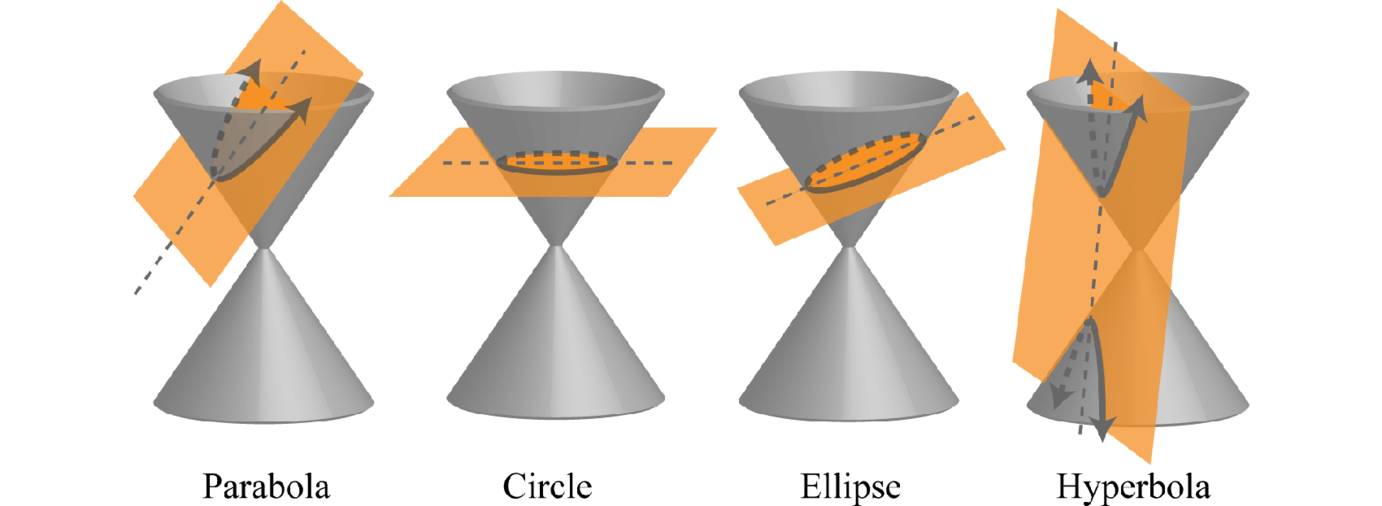
\includegraphics[width=0.6\textwidth]{stoznice.png}
\centering
\end{figure}

\section{Krožnica}

\[\{T(x,y) | d(T,S)=r\}\]

Enačba krožnice s središčem $S(p,q)$ in polmerom $r$ je $(x-p)^2+(y-q)^2=r^2$.\\

Potrebni pogoj $A=C$ in $B=0$. Zadostni pogoj $D^2+E^2>4AF$.

\begin{zgled}
    Napišimo enačbo krožnice s središčem $S(3,-7)$ in polmerom $r=3$.
\end{zgled}

\begin{zgled}
    Poiščimo krožnico, ki ima središče v $S(2,-3)$ in se dotika premice $x=4$. 
\end{zgled}

\begin{zgled}
    Pokažimo, da se krožnici $(x-8)^2+(y-6)^2=25$ in $(5x-16)^2+(5y-12)^2=25$ dotikata.
\end{zgled}

\begin{zgled}
    Iz diametralnih točk $A(-5,2)$ in $B(1,4)$ zapišimo enačbo krožnice.
\end{zgled}

\begin{zgled}
    \textcolor{red}{Določimo konstanto $k$, da bo $y=kx+2$ tangenta na $x^2+y^2=2$.} (vstavimo in iščemo le eno rešitev)
\end{zgled}

\fbox{\parbox{\textwidth}{Dopolnjevanje do popolnega kvadrata: $x^2+y^2-6x+4y+12=0$
\begin{enumerate}
    \item Združimo $x$ in $y$
    \item Če gre, izpostavimo člen pred $x^2$ in pred $y^2$
    \item Dopolnimo do kvadrata in uredimo, da cifra na desni, ostalo na levi
    \item Če gre, delimo enačbo z desno cifro, da imamo na desni $=1$
\end{enumerate}}}

\begin{zgled}
    Ali enačbi $x^2+y^2+8x-2y-8=0$ in $x^2+y^2+6y+10=0$ predstavljata krožnico. Če ja, napiši njen polmer in središče.
\end{zgled}

\begin{zgled}
    Napišimo enačbo krožnice, ki je očrtana trikotniku $ABC$ z oglišči $A(0,1), B(-2,-3)$ in $C(-3,-1)$.
\end{zgled}

\begin{example}
    NALOGE 228a, 229c, 231ac, \fbox{232adf}, 234a, 239a, 241a.
\end{example}

\section{Elipsa}

Elipsa je množica točk v ravnini, katerih vsota razdalj od izbranih točk $F_1$ in $F_2$ (gorišč) je konstantna.\\

V središčni legi $\frac{x^2}{a^2}+\frac{y^2}{b^2}=1$. $a$ in $b$ imenujemo velika in mala polos elipse, $A(-a,0),B(a,0),C(0,-b),D(0,b)$ so temena elipse, $F_1(-e,0)$ in $F_2(e,0)$ gorišči elipse, $e$ linearna ekscentričnost. Velja $e^2=a^2-b^2$ (če $a>b$) oziroma $e^2=b^2-a^2$ (če $b>a$).

\begin{figure}[H]
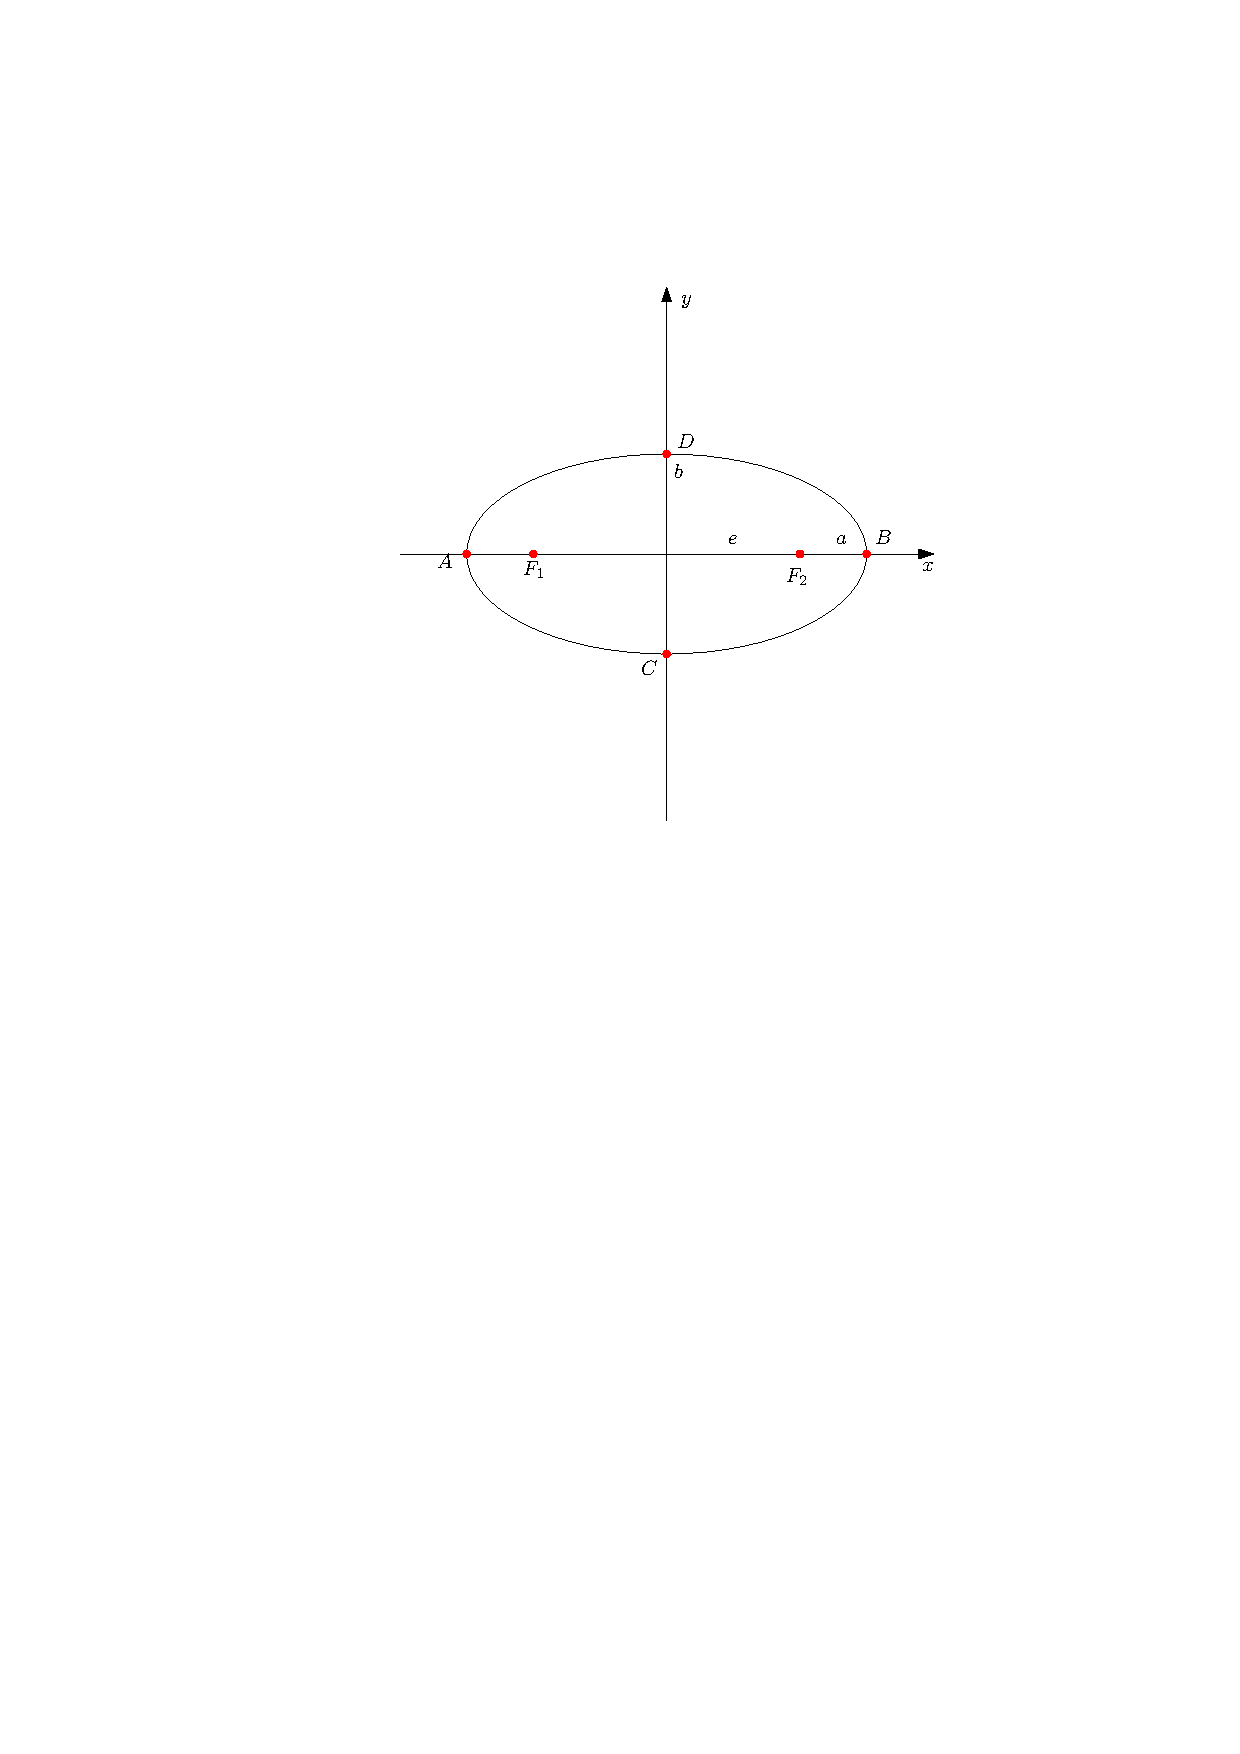
\includegraphics[width=0.5\textwidth]{stoznice.elipsa.pdf}
\centering
\end{figure}


\begin{zgled}
    Napišimo enačbo elipse v središčni legi, na kateri ležita točki $A(\sqrt{3},-\sqrt{10})$ in $B(-3,0)$. Zapišimo še njena gorišča.
\end{zgled}

V splošni legi $\frac{(x-p)^2}{a^2}+\frac{(y-q)^2}{b^2}=1$. Središče $S(p,q)$, temena in gorišča kot na sliki.

\begin{figure}[H]
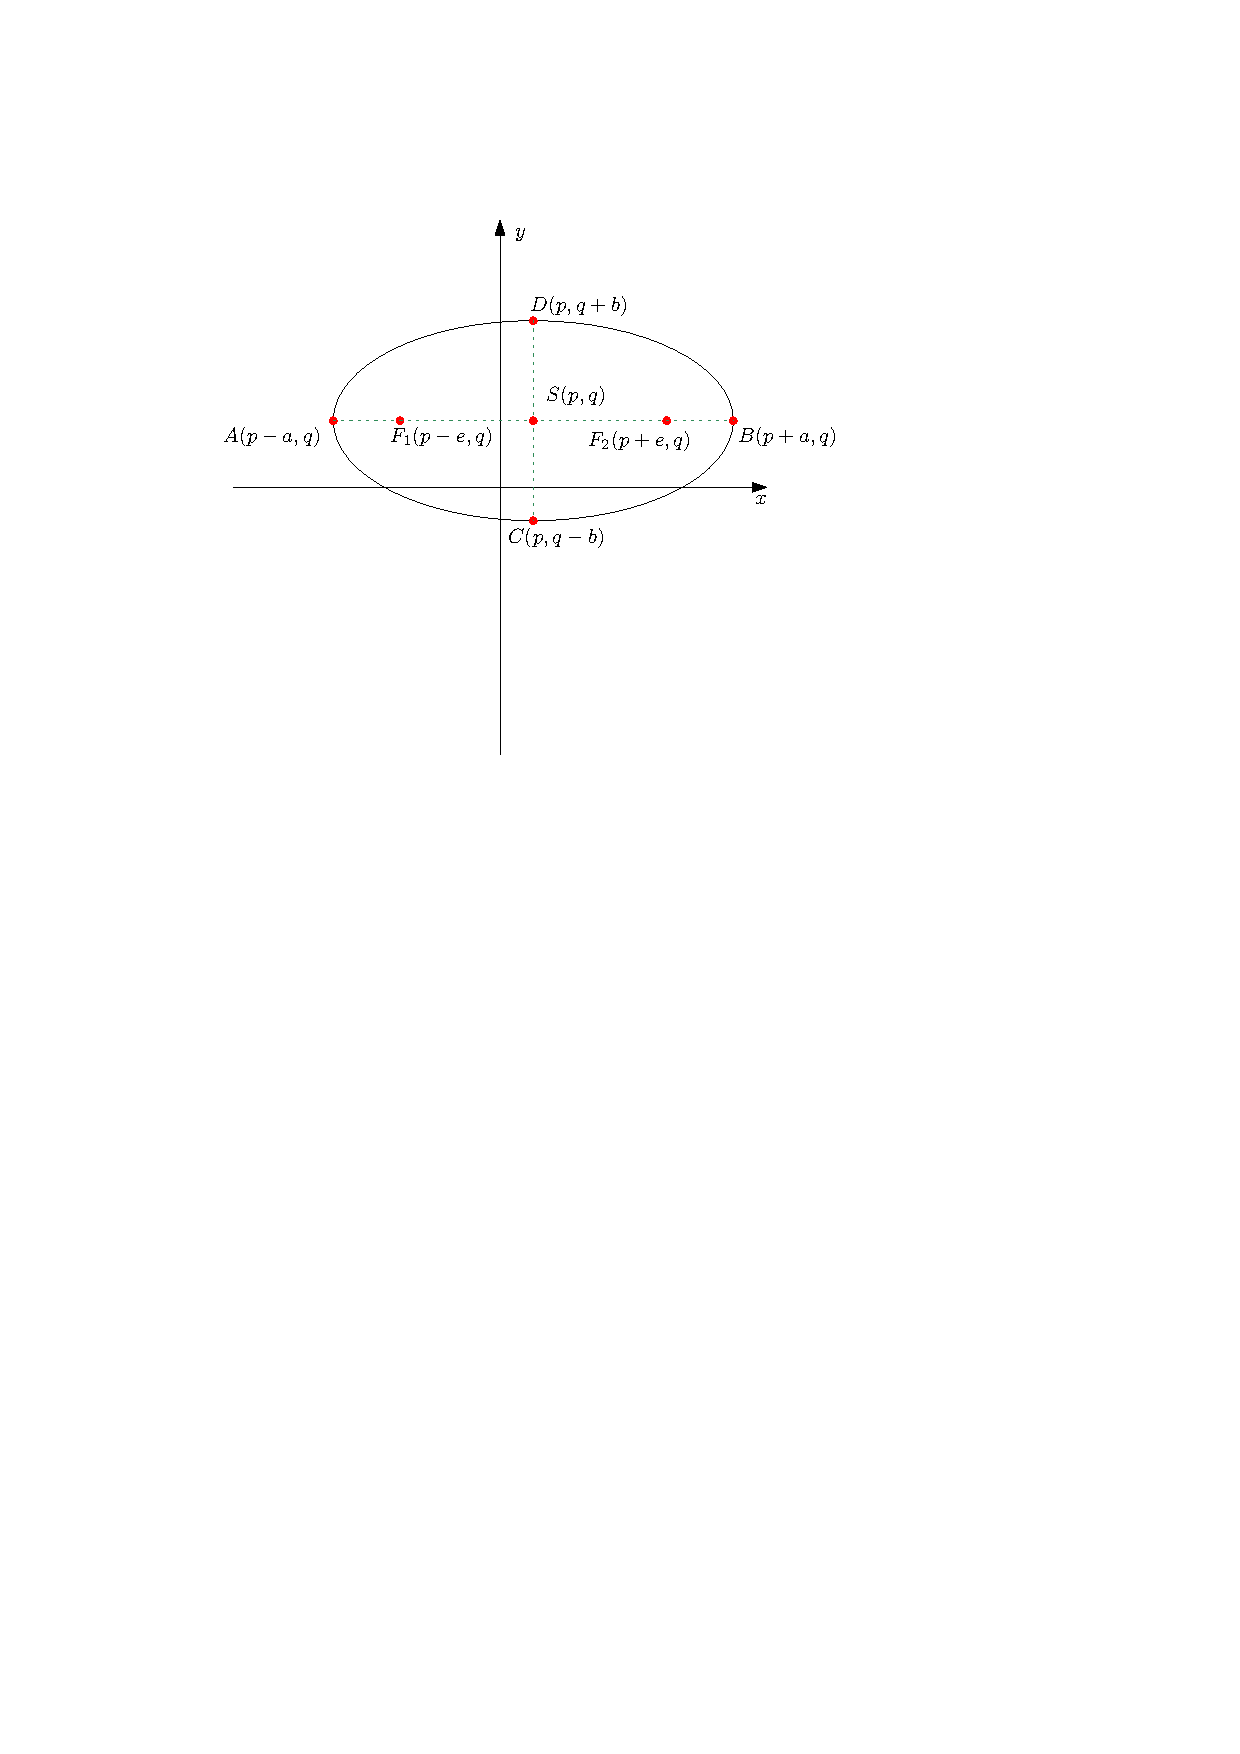
\includegraphics[width=0.6\textwidth]{stoznice.elipsa.splosna.pdf}
\centering
\end{figure}

\begin{zgled}
    Premaknimo enačbo elipse $5x^2+12y^2-60=0$, da bo imela središče v točki $S(3,-2)$ in zapišimo njeni novi gorišči.
\end{zgled}

\begin{zgled}
    Ali enačba $9x^2+4y^2+36x-8y+4=0$ predstavlja elipso. Če ja, jo narišimo in označimo simetrijske osi.
\end{zgled}

\begin{zgled}
    Ali enačba $4x^2+5y^2-4x+10y+6=0$ predstavlja elipso.
\end{zgled}

Potreben pogoj $A\neq C$ in $AC>0$

\begin{example}
    253ac, 257ab, 260a, \fbox{263ab nariši}, 266a, 272, 273.
\end{example}

\section{Hiperbola}

Hiperbola je množica točk v ravnini, katerih absolutna vrednost razlike razdalj od dveh izbranih točk (gorišč $F_1$ in $F_2$) je konstantna.

V središčni legi $\frac{x^2}{a^2}-\frac{y^2}{b^2}=1$. Glede na sliko, imenujemo $a$ glavna (ali realna) polos, $b$ imaginarna polos, $A(-a,0)$ in $B(a,0)$ temeni hiperbole, $F_1(-e,0)$ in $F_2(e,0)$ gorišči in $e$ linearna ekscentričnost, ki jo izračunamo kot $e^2=a^2+b^2$. Asimptoti sta premici $y=\pm\frac{b}{a}x$.\\
Hiperbola oblike $\frac{x^2}{a^2}-\frac{y^2}{b^2}=-1$ (oziroma $-\frac{x^2}{a^2}+\frac{y^2}{b^2}=1$) je ''podobna'', le da ''gleda gor-dol''. Enakoosa če $a=b$.

\begin{figure}[H]
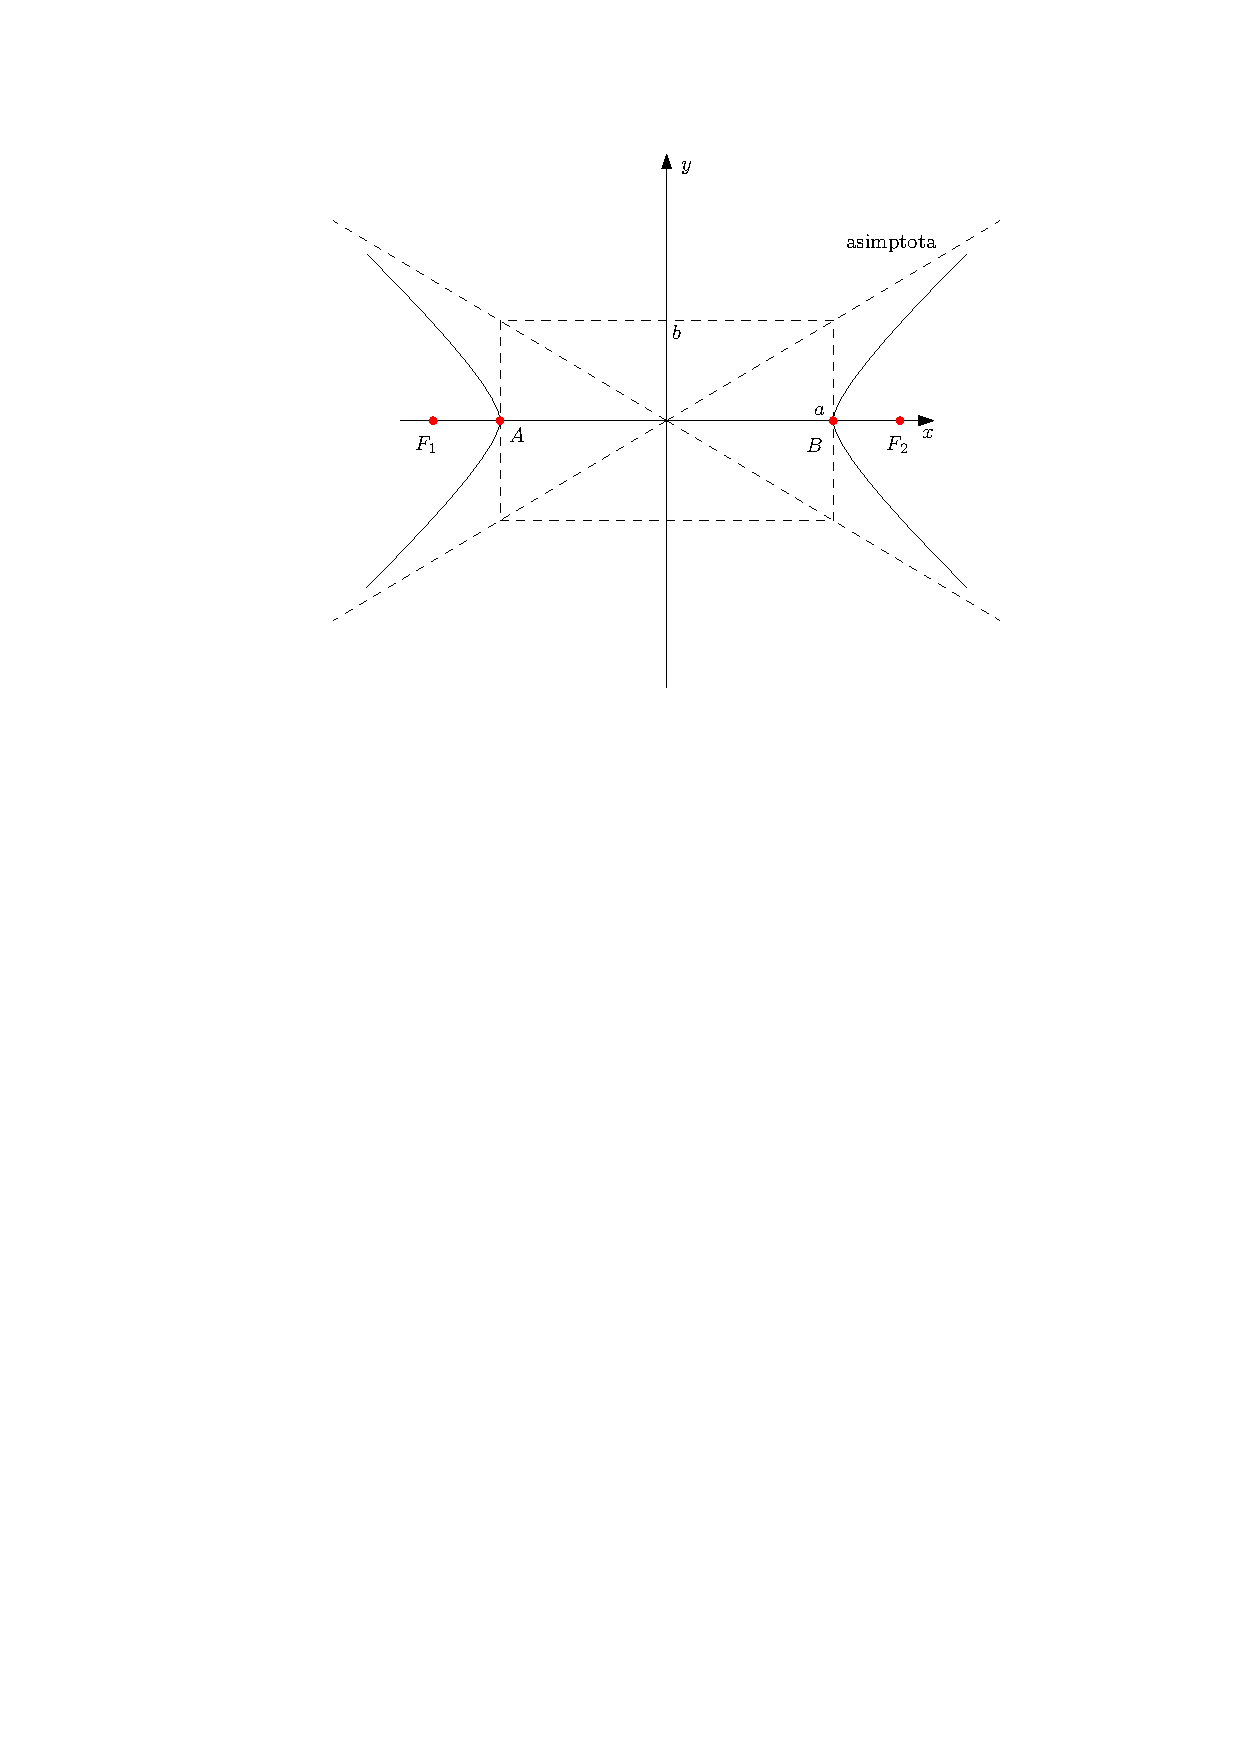
\includegraphics[width=0.6\textwidth]{stoznice.hiperbola.pdf}
\centering
\end{figure}

\begin{zgled}
    Zapišimo enačbo hiperbole v središčni legi, če poznamo njeno asimptoto $y=\frac{3}{2}x$ in vemo, da točka $A(2\sqrt{5},3)$ leži na njej.
\end{zgled}

V splošni legi $\frac{(x-p)^2}{a^2}-\frac{(y-q)^2}{b^2}=1$.

\begin{figure}[H]
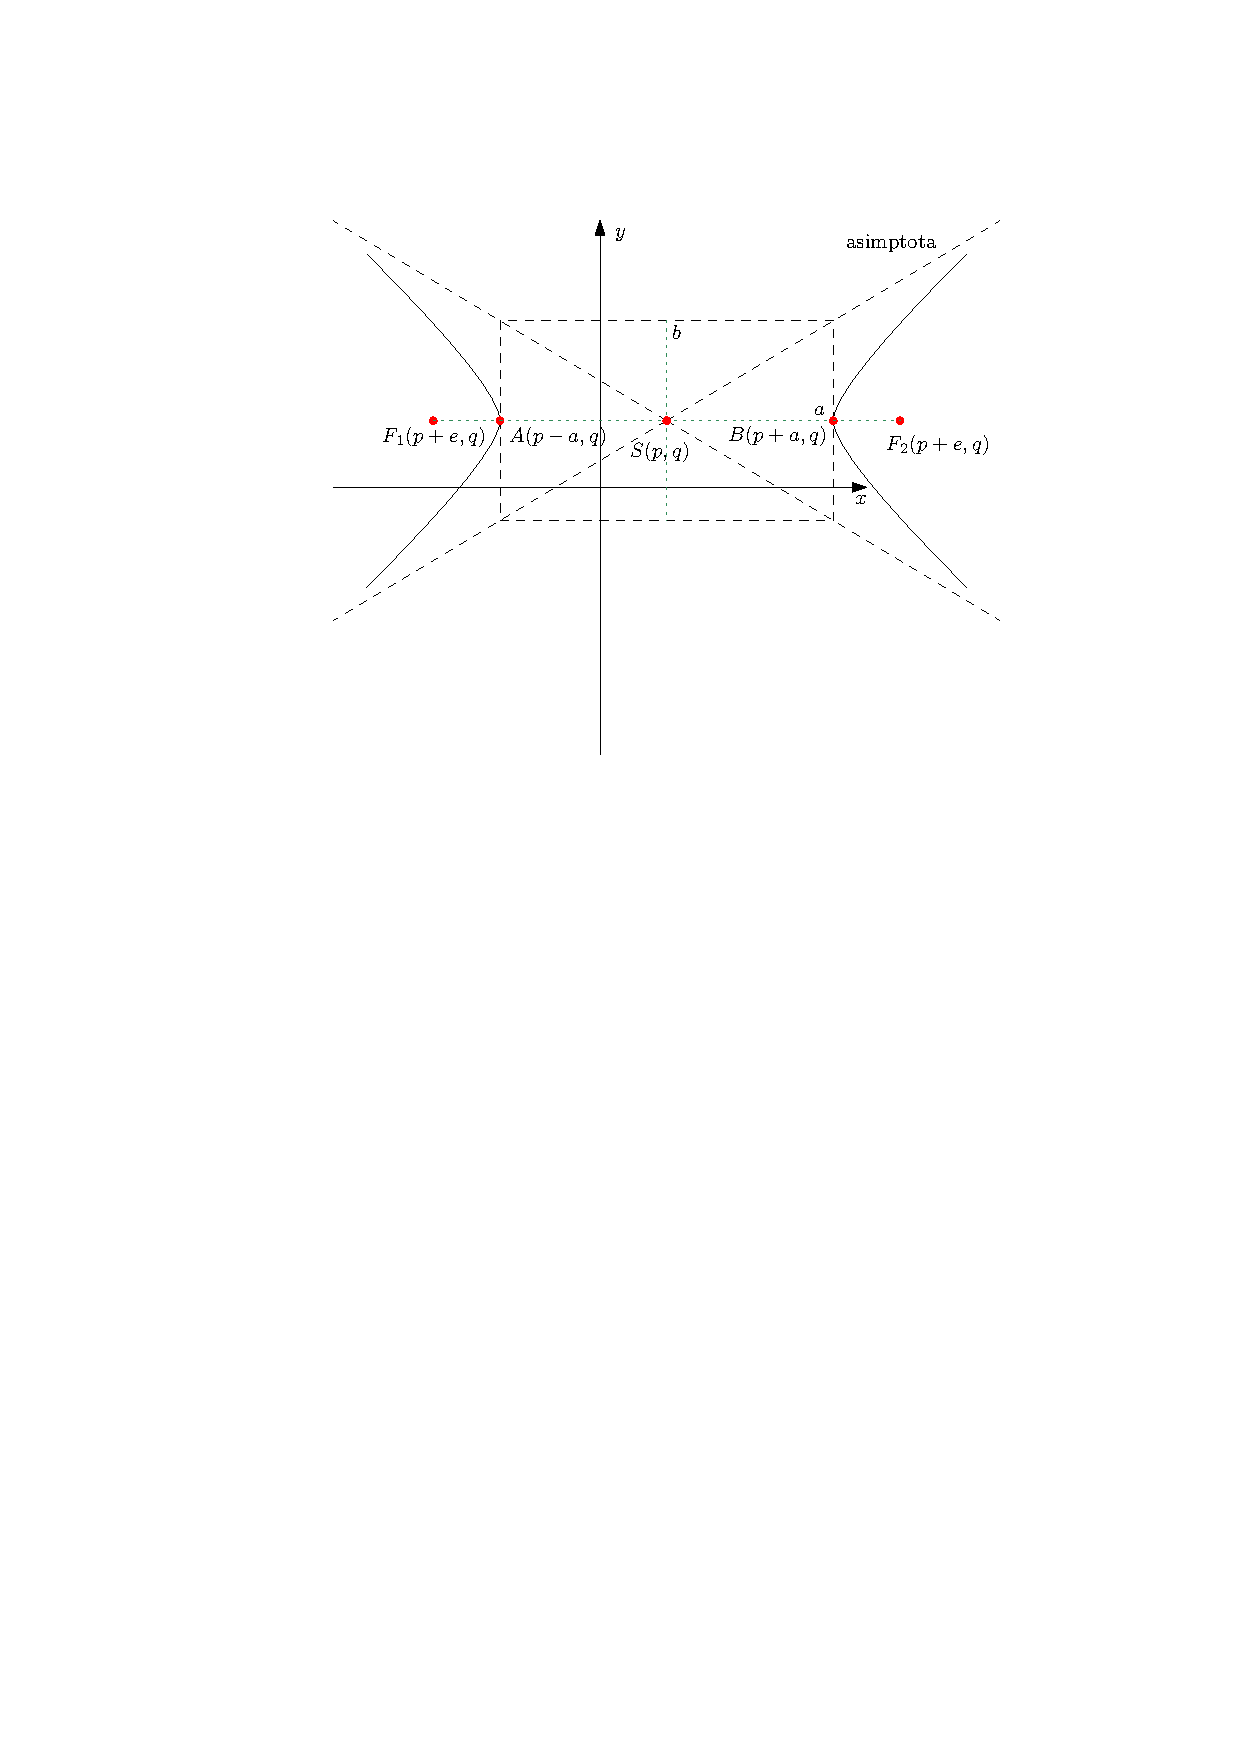
\includegraphics[width=0.6\textwidth]{stoznice.hiperbola.splosna.pdf}
\centering
\end{figure}

Potreben pogoj $AC<0$.

\begin{zgled}
    Izračunajmo gorišča, temeni, enačbi asimptot, simetrijske osi in narišimo hiperbolo $x^2-y^2-2x+4y-28=0$.
\end{zgled}

\begin{zgled}
    Nariši krivuljo $4x^2-9y^2+16x+18y-29=0$.
\end{zgled}

\begin{example}
    NALOGE 277ab, 278ac, \fbox{282}, \fbox{284ab}, \fbox{\fbox{286}}.
\end{example}


\section{Parabola}

Parabola je množica točk v ravnini, ki so enako oddaljene od izbrane točke (gorišče $F$) in izbrane premice (vodnica).\\

V središčni legi $y^2=2px$. Glede na sliko imenujemo $A(0,0)$ teme parabole, $p=2|OF|$ parameter parabole, $F(\frac{p}{2},0)$ gorišče, enačba premice vodnice pa je $x=-\frac{p}{2}$.

\begin{figure}[H]
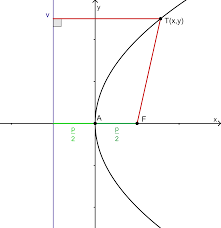
\includegraphics[width=0.5\textwidth]{stoznice.parabola.png}
\centering
\end{figure}

\begin{zgled}
    Zapišimo enačbo parabole, ki ima gorišče v $F(4,0)$ in teme v koordinatnem izhodišču.
\end{zgled}
\begin{zgled}
    Zapišimo enačbo parabole v izhodiščni legi, na kateri leži točka $T(3,-2)$.
\end{zgled}
\begin{zgled}
    Zapišimo točki parabole $y^2=12x$, ki sta od gorišča oddaljeni za 7 enot.
\end{zgled}

V splošni legi $(y-q)^2=2p(x-t)$. Potreben pogoj $AC=0$, a ne oba hkrati. V tem primeru $F(\frac{p}{2}+t,q), x=-\frac{p}{2}+q, T(t,q)$.

\begin{zgled}
    \textcolor{red}{Narišimo parabolo, če vemo, da je njeno teme $T(-2,-6)$ in gorišče $F(4,-6)$.}\textcolor{green}{}
\end{zgled}
\begin{zgled}
    \textcolor{red}{Preveri ali $y^2-6x-10y-15$ predstavlja parabolo. Zapiši teme, gorišče, enačbo vodnice ter presečišča s koordinatnima osema.}\textcolor{green}{}
\end{zgled}

\begin{example}
    289vse, 300a, 301b, 302a, \fbox{304vse}, \fbox{306a}
\end{example}

\section{Presečišča stožnic}
\begin{zgled}
    Izračunajmo presečišča $x^2+y^2=8$, $x^2+3y^2=12$.
\end{zgled}

\begin{zgled}
    Izračunajmo presečišča $x^2-2y^2=125$, $y^2=10x$.
\end{zgled}

\begin{zgled}
    Izračunajmo presečišča $(x-2)^2+(y+3)^2=14$, $(x+\frac{1}{2})^2+(y+\frac{1}{2})^2=\frac{13}{2}$.
\end{zgled}

\begin{zgled}
    Izračunajmo presečišča $y^2=2x$, $2x-y-6=0$.
\end{zgled}

\begin{zgled}
    Izračunajmo presečišča $4x^2+5y^2=20$, $4x^2-y^2=36$.
\end{zgled}

\begin{example}
    \fbox{309ab}cd, \fbox{310a}, \fbox{311ab}.
\end{example}

\end{document}